\chapter{Mission}

\section{Sujet du stage}
%Vous présentez le sujet initial tel qu'il a été validé, ses éventuelles évolutions (et leurs causes). Attention, si votre sujet a fortement évolué, vous devez en référer à votre suiveur (éventuellement il devrait être re-validé).
Le sujet de mon stage était la prise en charge du suivi, de la gestion et de l'optimisation  du \gls{reporting} des différents tests de l'équipe \gls{TC}. 
En effet, chaque rapport de test se décompose en plusieurs étapes de test, qui sont toutes reliées à des exigences du cahier des charges. Pour chaque test, QDVC et ICE déterminent si oui ou non les résultats permettent de considérer le rapport comme accepté. Ainsi chaque rapport constitue une preuve nécessaire à la validation des exigences et sans laquelle le système ne peut être validé. 
Chaque rapport est édité et consigné dans la base de donnée \gls{SnagR}. 
Cependant, cet outil est initialement destiné aux projets de génie civil et à la gestion des problèmes d'installation, c'est pour cela que l'utilisation de cet outil a été réduite à l'édition de rapports de test peu de temps après mon arrivée.
Ainsi la problématique initiale fût : Comment suivre efficacement la production et la validation des rapports ?

%Resituer votre sujet dans les objectifs de l'entreprise.
%Avez-vous repris un travail existant ?
%Aviez-vous un cahier des charges précis ou bien avez-vous contribué à son élaboration ?

\section{Planning}
%Vous pouvez présenter le planning initial et le planning réel avec les dates importantes.
En terme de délais, il m'a fallu incorporer les différentes solutions que j'ai mises au point au fur et à mesure du projet, tout en proposition une version finale environ un mois avant la fin de mon stage afin de pouvoir suffisamment l'éprouver.
%Quelles ont été les étapes importantes ? Indiquez celles qui auraient été les plus difficiles, les plus intéressantes, etc.
Le but à court terme était de mettre en place un processus efficace de traitement des rapports et de leurs données puis de l'intégrer au fonctionnement global du projet.
Dans un second temps, le but à long terme était d'automatiser une partie de ce processus, notamment l'extraction et le traitement des données des rapports. 
Enfin, au cours du dernier mois, il m'a fallut former mon remplaçant tant au fonctionnement du \gls{reporting} qu'à l'utilisation des différents outils que j'ai créé.
Chacune de ces trois grandes étapes comporte son lot de difficultés :
\begin{itemize}
\item \textbf{L'initialisation du processus :} L'ampleur du projet constitue une première difficulté. En effet, la tâche qui m'a été confiée demande une bonne connaissance non seulement du fonctionnement interne du projet mais aussi de l'état actuel de son avancement.
\item \textbf{Son automatisation :} La base de donnée avec laquelle je travaillais n'avait pas été documenté, ainsi l'extraction de données s'est avérée complexe.
\item \textbf{Sa transmission :} Former quelqu'un tout en continuant à travailler a constitué un réel défis pour quelqu'un sans expérience professionnelle. 
\end{itemize}
\section{Contributions}
%Quel était l'état du projet à votre arrivée ? et à la fin ?
À mon arrivée, l'installation était arrivée à un stade suffisamment avancé pour permettre de débuter les phases de test (et cela depuis quelques mois).
Ainsi la production des rapports était tout juste amorcée.
C'est pour cela que le projet de mon stage a commencé au moment où on me l'a confié.
À la fin de mon stage, la phase de test était avancée à plus de 50\% et le processus de production et des suivi des rapports de test était en place et fonctionnel.
%Avez-vous travaillé seul ou avec d'autres ? Quelles ont été vos contributions exactes ?
Mes managers m'ont transmis la documentation nécessaire à l'initialisation, de mon projet puis m'ont guidé au cours du stage afin de me permette d'y apporter des améliorations et de nouvelles fonctionnalités. 
Chaque semaine je me devais d'envoyer un rapport sur l'avancement du \gls{reporting} à différents manager Thalès ainsi qu'au client (QDVC).
Ces rapports avaient pour fonction l'aide à la décision et comportaient de nombreux indicateurs d'avancement (\gls{KPI} : Key Progress Indicator).
Je travaillais conjointement avec :
\begin{itemize}
\item Le service de gestion des documents afin de gérer l'indexation des rapports ainsi que leur mise en ligne sur \gls{Mezzoteam} et \gls{e-TOL}.
\item Le service informatique de QDVC afin de proposer des amélioration de la base de données SnagR mais aussi pour leur faire remonter les différentes erreurs de l'interface web.
\item L'équipe \gls{RAMS}  (en français : Fiabilité Maintenabilité Disponibilité et Sécurité), chargée de la sureté de fonctionnement, afin d'effectuer le suivi de la production des documents permettant de prouver la conformité du système en terme de sécurité.
\item L'équipe d'ingénieurs Système, qui est responsable du design, avec qui j'ai étudié différentes exigences.
\item L'équipe d'ingénieurs \gls{TC} afin d'identifier les différents facteurs bloquants ralentissant la production des rapports.
\end{itemize}

%Avez-vous réalisé une étude, une maquette, une preuve de concept, un produit ou une application complète ? Que reste-t-il à faire pour rendre utilisable votre travail ?

En parallèle de ces différentes activités, il m'a fallut automatiser l'extraction des données des rapports. Pour cela j'ai développé un script permettant de se connecter au site \gls{SnagR}, d'en extraire différents lots de données et de les exporter dans différents fichiers Excel. Il m'a fallut aussi ajouter à cette application une fonctionnalité de sauvegarde complète de rapports, en cas de problème avec les serveurs SnagR, serveurs auquel Thalès n'avait pas accès physiquement. 
Ce script est exécutable à travers l'invite de commande, et comme nous le verrons plus tard j'ai formé la personne me remplaçant à son utilisation mais j'ai aussi préparé une documentations. Ainsi, à mon départ, mon remplaçant utilisait déjà les résultats de mon travail.

\section{Technologies}
%Quels sont les outils, environnements ou logiciels que vous avez utilisés ?
Durant mon stage, j'ai donc utilisé : 
\begin{itemize}
\item \textbf{Pour le développement :}
\begin{itemize}
\item \textit{Comme langage de programmation :} Python 2.7 puis Python 3.7.
\item \textit{Comme environnement de développement :} PyCharm, \gls{IDE} de la suite IntelliJ, développé par JetBrains.
\end{itemize}
\item \textbf{Pour la bureautique :} La suite Microsoft Office, plus particulièrement Excel, pour la communication et l'échange d'informations internes au projet, et TexMaker, un éditeur de documents \gls{LaTeX}, pour la rédaction de ce rapport.
\item \textbf{Pour la gestion de mes tâches :} Trello, une solution en ligne de gestion de projet s'inscrivant dans le cadre des \gls{methodesagiles}.
\item \textbf{Pour la gestion des différentes versions du script :} La technologie \gls{Git}, en utilisant l'hébergeur GitHub.
\end{itemize}

%Quelles sont les méthodes utilisées dans votre équipe ? (eg. méthode agile...)
Au sein de l'équipe \gls{TC}, les \gls{methodesagiles} ont été utilisées notamment par le biais d'outils comme \gls{SnagR} ou Jira Ops. En effet, \gls{SnagR} permet aussi de répertorier les problèmes ou points bloquants que les différentes équipes du projet rencontrent. 

\gls{SnagR} est la solution choisie par le Consortium, mais pour son fonctionnement interne, Thales a choisit d'utiliser Jira Ops , qui permet à l'équipe inshore de faire remonter les différents problèmes rencontrés à l'équipe offshore, sous forme de \gls{PCR}.

Parmis ces trois outils que sont SnagR, Jira Ops et Trello \footnote{Jira Ops et Trello sont d'ailleurs édités par la même entreprise : Atlassian} SnagR et Trello intègrent les \gls{methodesagiles}, et plus particulièrement la méthode \textit{KanBan}.

\textbf{La méthode Kanban,} est une méthode de gestion de projet où chaque tâche est placée sur une carte et chaque carte doit être placée dans un tableau. Chaque carte peut être assignée à un ou plusieurs utilisateurs et on peut lui attribuer une date d'échéance ainsi qu'une ou des étiquettes permettant de catégoriser la tâche associée. L'avancement d'une tache est représenté par le déplacement de la carte à laquelle est est liée d'un tableau à un autre. 
En ce qui concerne mon organisation personnelle avec Trello, j'ai utilisé 5 tableaux :
Tâches récurrentes, À faire, En attente, En cours et Fait. Les taches portant l'étiquette "Récurrente" (étiquette rouge dans l'exemple ci-dessous) suivent le développement 


Il est basé sur une organisation des projets en planches listant des cartes, chacune représentant des tâches. Les cartes sont assignables à des utilisateurs et sont mobiles d'une planche à l'autre, traduisant leur avancement. 

Voici ci-dessous, l'interface de Trello puis celle de SnagR.

\begin{center}
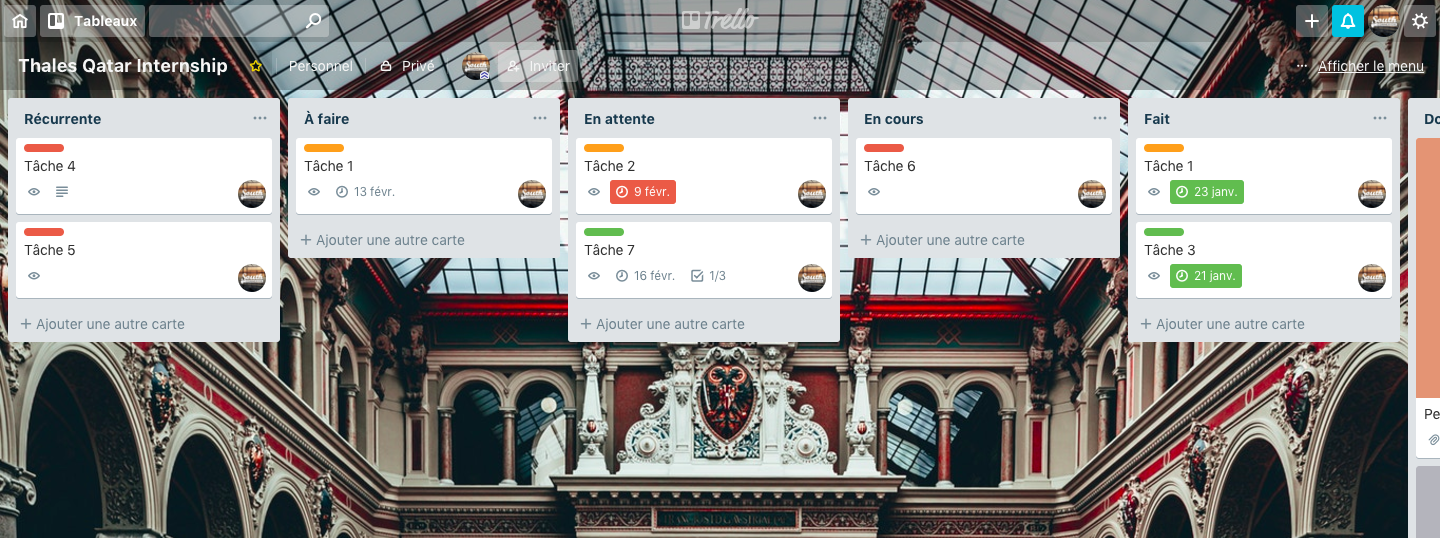
\includegraphics[height=5.5cm]{ressources/images/figures/Trello.png}

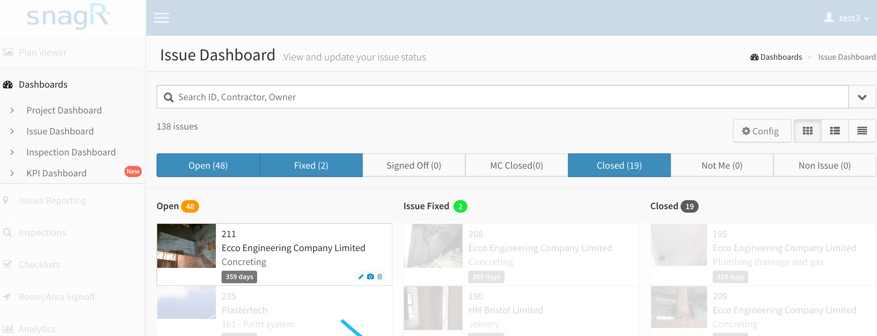
\includegraphics[height=5.5cm]{ressources/images/figures/SnagR.jpeg}
\end{center}


%Comment les développements ont été vérifiés/testés/validés ?
MOI

%Quelles sont les technologies utilisées pour le projet ? Il ne s'agit pas de faire de longs développements ici mais de présenter une synthèse.

\section{Prise de recul}
%Quel a été l'intérêt de votre travail pour l'entreprise ? Que va devenir votre contribution ? Présenter les perspectives.
%Quelles sont les améliorations à envisager ? Quelle est la maintenance à prévoir sur cette réalisation ou cette application ?
%Selon les cas, présentez vos réflexions sur l'impact de votre travail sur les utilisateurs, les nouveaux usages, le respect de la vie privée ou de l'environnement...